
\documentclass[main.tex]{subfiles}

\begin{document}

\chapter{Pull-Out}
\label{LEC:PullOut}

\paragraph{Outline:}
In this chapter we introduce elementary test setups for the pullout of a bar from a cementitious matrix.
\mnote{Test setup and structural response}
The goal is set up the playground for questions of test design. Tests are mostly focusing on isolated
effects of material behavior, like debonding between two material components. However, it is seldom possible
to completely avoid additional effects. The pull-out test setup can be conveniently used to demonstrate 
the dilemmas involved in a test setup design. By raising these questions we shall motivate the 
deeper look at the material behavior versus the structural behavior in Chapter \ref{LEC:BondBehavior}.

\paragraph{Addressed questions:}
\begin{itemize}
\item 
How to identify a bond law describing the bond behavior between matrix and reinforcement? 
\item How to design a test for the calibration of the bond characteristics? 
\item What kinds of tests exist? What are their advantages and disadvantages?
\item Which tests are appropriate for the different types of reinforcement? (steel, carbon/glass fiber-reinforced polymer,
carbon or glass textile fabrics reinforcement. 
\end{itemize}

\section{Pullout test setup}
\label{Pullout_test_setup}

\mnote{First standardized pullout test}
The development of a test suitable for characterization of the bond behavior between a reinforcing steel bar and concrete matrix dates back to sixties. The RILEM-FIB-CEB recommendation test has been proposed in 1973. Fig.~\ref{fig_pull-out_rilem} shows the prescribed boundary conditions and measuring equipment that records the pull-out curve in terms of the pull-out force versus slip displacement of the bar at the loaded $s_l$ and unloaded $s_u$ free ends. The loading process is controlled by the prescribed pullout displacement and the corresponding force is recorded. In this way, also pullout curve with diminishing force after the peak value can be measured.

\begin{figure}[tbh]
	\centering
	\begin{subfigure}{0.45\textwidth}
	\centering
  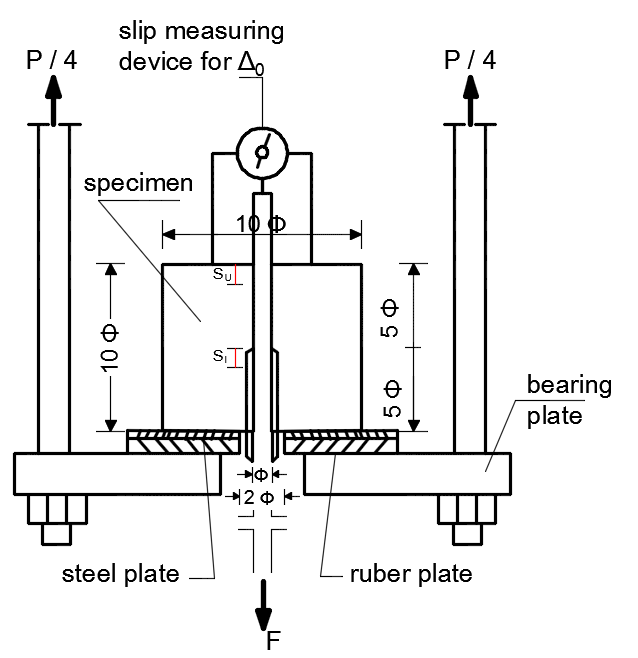
\includegraphics[width=7cm]{fig/Lecture02/_300___pullout.png}
	\end{subfigure}
	\begin{subfigure}{0.45\textwidth}
	\centering
  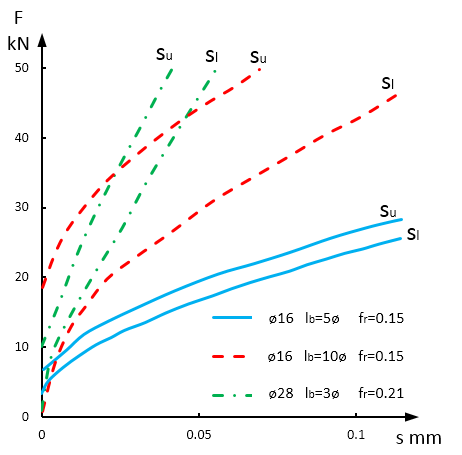
\includegraphics[width=7cm]{fig/Lecture02/_300___pullout-rilem.png}
	\end{subfigure}
	\caption{RILEM pull-out test to characterize the bond between steel and concrete.}
	\label{fig_pull-out_rilem}
\end{figure}
The curves displayed in right diagram of Fig.~\ref{fig_pull-out_rilem} exemplify 
two observations that can be made using this test setup:
\begin{itemize}
    \item The pullout curve strongly depends on the embedded length and on the diameter of the bar.
    \item The displacement measured at the loaded and unloaded end differ and this difference is strongly affected by the embedded length.
\end{itemize}

Obviously, the experimentally observed trends must be governed by the principles of physics and mechanics. It is our ambition to capture the underlying phenomena of the bond behavior with the goal to predict the  pullout behavior for changed test parameters. 

\mnote{Derived pull-out tests}
But before approaching a more fundamental view to the effects governing the bond behavior let us span the scope of the bond description to other materials and other types of test setup. 
A similar type of the pullout test setup has been used to test the behavior of nonmetallic reinforcement as exemplified in Fig.~\ref{fig:gfrp_pullout}.
Notice that in both mentioned pullout test setups, the bond zone is located inside the specimen and 
there is a bond-free zone of a predefined depth starting at the loaded side. This bond-free zone is introduced with the goal to render uniform material properties along the tested bond length and to avoid the effect of a boundary zone.
\begin{figure}[tb]
	\centering
  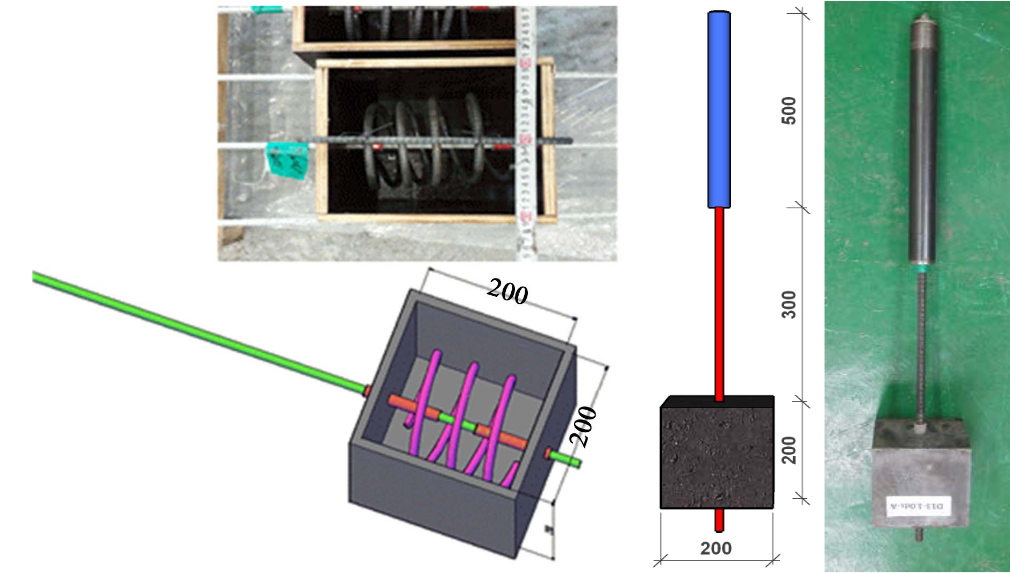
\includegraphics[width=10cm]{fig/Lecture02/gfrp_pullout.png}
	\caption{Pullout of GFRP bar from the concrete matrix.}
	\label{fig:gfrp_pullout}
\end{figure}

\mnote{Undesired compression}
The described pullout test setup is very common in practice, primarily to
its simplicity. However, it is not ideal in all situations
because it does not really correspond to the situation in the structural elements.
The reason is that due to the placement of supports at the loaded side of the
specimen, non-negligible compressive
stresses develop within bond zone of the concrete matrix. 
Such a stress state does not represent the state 
in the bond zone of a structural element which is mostly
loaded in tension. As documented by experimental studies, e.g. in \cite{de2008bond}
the effect on the bond behavior is significant.

\mnote{Beam anchorage test}
The refined setup for bond characterization has been proposed 
in the form of beams or beam-end-sections as exemplified Fig.~\ref{fig:pull-beam_end_test}.
Apparently, this test configuration is closer to the condition of a crack in a tensile zone of 
a structural specimen. The pullout displacement is measured as the opening of the crack. 
The test is controlled by 
the vertical displacement and the corresponding load is measured. 
It is important to note that the debonding propagates in both directions. 
Symmetry of the debonding process is provided until the ultimate load has been achieved. Once 
the pullout force has been reached at one side, the process becomes non-symmetric.
As we shall discuss later on, this might become a problem in cases of 
materials that exhibit a so called bond softening. However, in case of steel rebars
this test configuration provides a suitable solution.
\begin{figure}[tb]
	\centering
	\begin{subfigure}{0.48\textwidth}
	\centering
  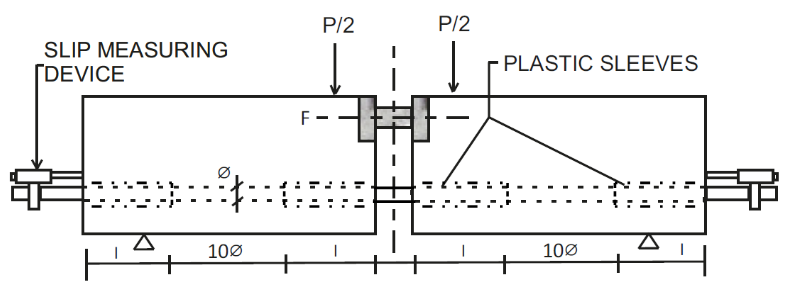
\includegraphics[width=8.3cm]{fig/Lecture02/_300___beam-pullout-test.png}
	\end{subfigure}
	\begin{subfigure}{0.48\textwidth}
	\centering
  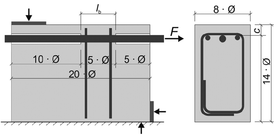
\includegraphics[width=5cm]{fig/Lecture02/beam_end_test.png}
	\end{subfigure}
	\caption{Beam tests focused on the bond characterization.}
	\label{fig:pull-beam_end_test}
\end{figure}

\mnote{Beam-end test}
Further step in the development of experimental methods for the bond characterization is depicted in Fig.~\ref{fig:pull-beam_end_test}; right showing the beam-end test. Its boundary conditions, i.e. the placement of supports and loading are designed with the goal to render the stress state equivalent to the end zone of a tensile reinforcement in a beam. It aims to combine the positive features of both the pull-out test and of the beam anchorage test.  

\begin{figure}[tb]
	\centering
	\begin{subfigure}{0.45\textwidth}
	\centering
  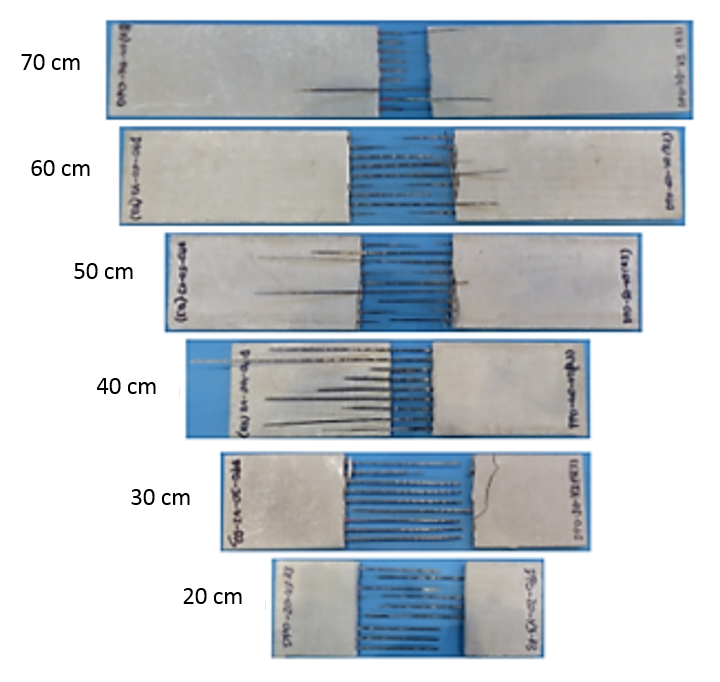
\includegraphics[width=5cm]{fig/Lecture02/_300___failure_modes.png}
	\end{subfigure}
	\begin{subfigure}{0.5\textwidth}
	\centering
  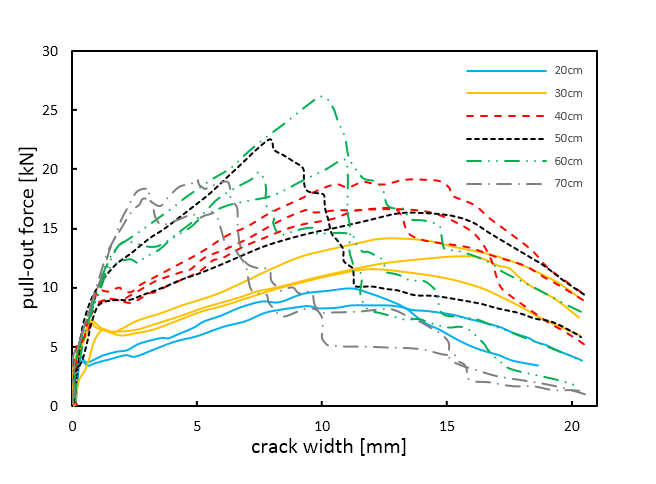
\includegraphics[width=8cm]{fig/Lecture02/_300___test_carbon.png}
	\end{subfigure}
	\caption{Double sided pullout test applied to carbon textile fabrics.}
	\label{fig:double_sided_po_test}
\end{figure}


\mnote{Test setups for fine-scale reinforcement}
In case of flexible, fine scale reinforcement further types of test setups 
for bond characterization have been developed. An example of such a test is 
shown for testing the pullout behavior of textile fabrics. An example in Fig.~\ref{fig:double_sided_po_test} shows a test series performed on 
double sided pullout test of textile fabrics. The planar test specimens
were clamped using steel plates positioned near to the middle section 
containing a notch and pulled apart. The opening of the notch that we refer to as crack opening displacement (COD) was recorded during the test. This test setup can be seen in analogy 
to the beam anchorage length rendering a symmetric debonding on both sides up to the maximum
pullout force. From there on, the process becomes non-symmetric. This fact makes it impossible
to characterize the bond in material exhibiting a so called softening, i.e. decreasing shear
for increasing slip after the peak value. Up to the peak, the end slip 
can be assumed as a half of the crack-opening displacement $s = COD/2$. 

\begin{figure}[tb]
	\centering
  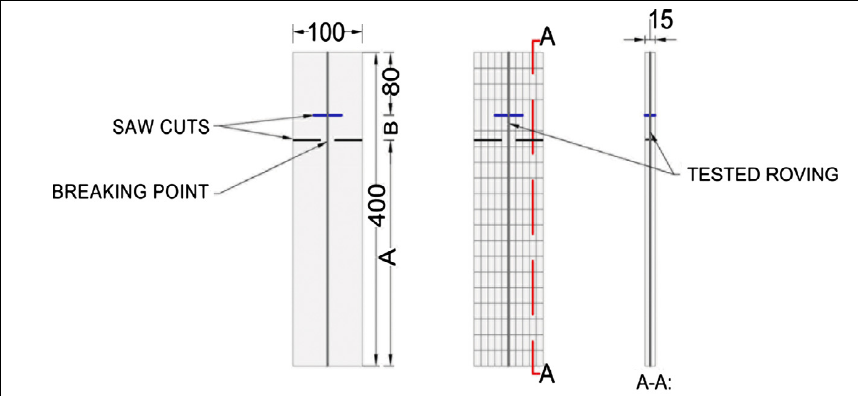
\includegraphics[trim={1mm 1mm 1mm 1mm},clip,width=8cm]{fig/Lecture02/pullout_with_cut.png}
	\caption{Double sided pullout test for a single fiber with a predefined pullout length at one side
	using a cut at one side.}
	\label{fig:pullout_with_cut}
\end{figure}

To cover also the bond behavior exhibiting softening, a small-scale test 
setup depicted in Fig.~\ref{fig:pullout_with_cut} has been proposed. 
This test setup has been derived from the double sided test setup with the 
goal to prescribe which side will start debonding. This test setup demonstrates
the dilemma involved in the pullout test design. The stress profile should be
as close as possible to the condition of crack bridge.
Let us remark, that
the test response must be treated with care as it contains the transition
from a symmetrical debonding to a non-symmetrical one.

The brief survey of test setups demonstrates the existing variety of 
characterization methods that are specialized for individual types of 
materials. The purpose of this survey is to motivate a unified
view to these experimental setups using the objective description of the bond behavior that 
is independent on the particular test configuration. 
The theoretical description of the correspondence between the 
local bond behavior and the global (structural) response of the pullout test
is a must for a sound and detailed interpretation of experimental data.

\paragraph{Question:}
The double sided pullout test includes two debonded zones. 
Can we simply say that the whole process is symmetric and just 
calculate the pullout displacement at one side by setting $w = COD/2$?


\section{Objectivity of a material model}

The bond-slip law represents an objective material property characterizing the material behavior at any point within the interface. 
Fig.~\ref{FIGDrawingStructureMaterial} shows the bond-slip law $\tau(s)$ defining the material behavior at any material point $x$ along the embedded length. 

The structural behavior that is measurable as a force-displacement relationship is represented by the  pull-out curve  $P(w)$ relating 
the displacement of the loaded fiber or reinforcement end with the applied pull-out force.
Given a continuous slip $s(x)$ along the interface we can visualize the pullout force $P$ as the green area representing the integral 
\[
P = \int_{0}^{L} \tau(s(x)) \, \mathrm{d}x.
\]

By identifying a "true" bond-slip law we get the possibility to predict the pull-out curve for diversity of loading scenarios. It is the key to the prediction of structural response. The question is how to identify the bond slip law from an experimental observation, e.g. from the measured pull-out curve $P(w)$.

\begin{figure}[ht]
	\centering
  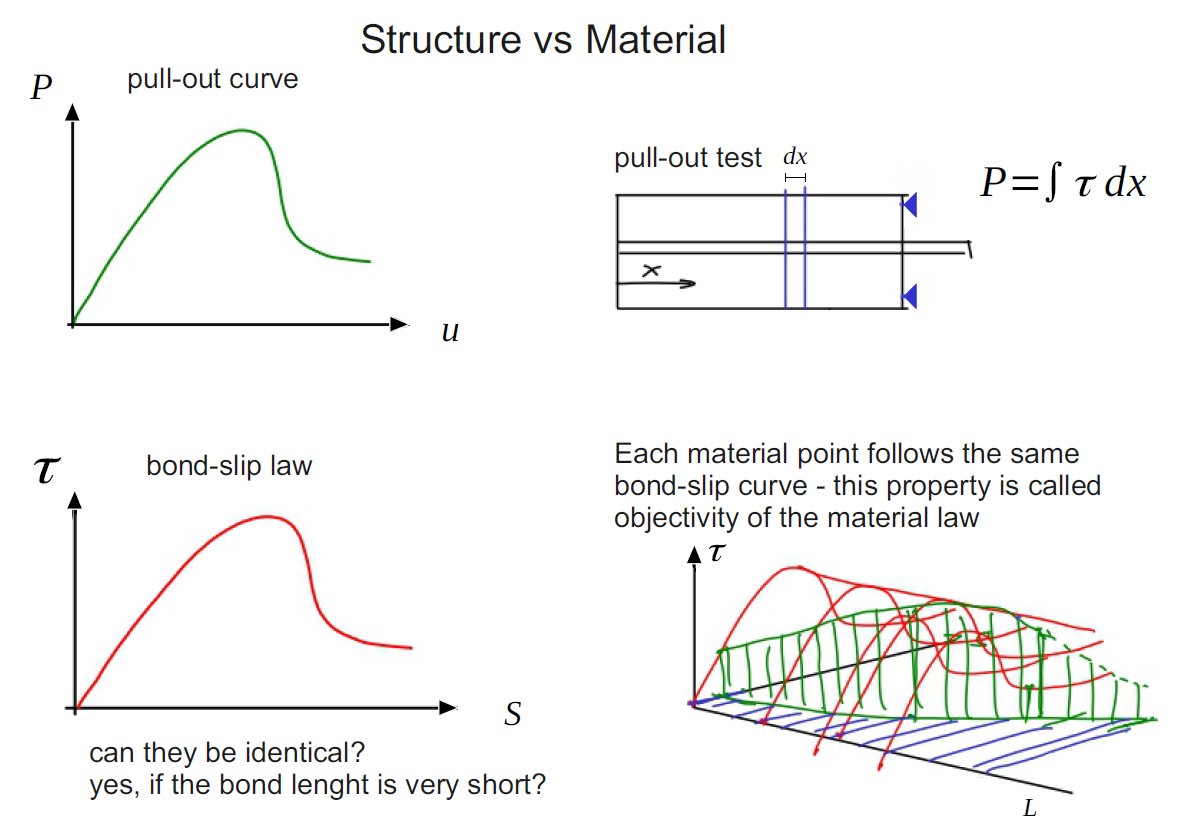
\includegraphics[width=0.7\textwidth]{drawings/structure_versus_material.png}
	\caption{Relation between material behavior and structural behavior}
	\label{FIGDrawingStructureMaterial}
\end{figure}

A simple experimental strategy to identify the bond slip law attempts to use a very short embedded length with the goal to achieve a uniform slip along the whole interface length. Then, the front and end slip of the pullout test are the same. In such a case, the pull-out curve can be directly transformed to the bond-slip relation by dividing the force with the interface area given as the product of the perimeter $p$ and length $L$ 
\[
\tau(s) =  \frac{1}{pL} P(s).
\]
However, it is rather difficult to design such a short test setup in a reproducible way. The short section of the material along the interface zone exhibits a relatively large scatter of properties so that many tests have to be conducted. Furthermore, the production of small size specimens results in a material behavior that is different from the \textit{in-situ} conditions. 

Realistic prediction of the pullout behavior is needed to support both the efficient and goal oriented material design with tuned material behavior. 
At the same time, it provides a valuable input for the formulation of design codes. In the sequel we will exemplify this issue on the example of the identification of the anchorage length. 

The structural configuration of the pullout test is depicted in  Fig.~\ref{fig_pull-out_rigid_matrix}, including the elastic parameters of the material components. The Figure also shows the boundary conditions BC1, BC2 that can be considered to solve the pullout test. The boundary condition BC3 with the clamped reinforcement represents a configuration of a crack bridge in a tensile test that we will discuss in the context of a multiple cracking behavior of brittle-matrix composites.

\saeed{can I add Parameters'(Lb, Lf, A, E, etc.) definition on the right side of the figure?}

\begin{figure}[ht]
	\centering
  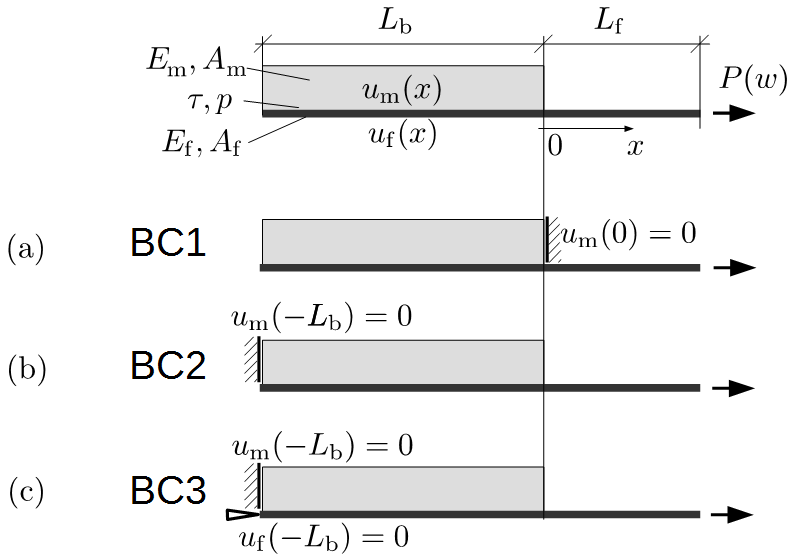
\includegraphics[width=10cm]{fig/Lecture02/figure_pullouts.png}
	\caption{One dimensional idealization of the pullout test as boundary value problem}
	\label{fig_pull-out_rigid_matrix}
\end{figure}
All the displayed configurations can be associated with different types of material behavior. If we assume rigid matrix and constant or linear bond-slip law, it is possible to derive analytical solutions of the pullout problem.

In case of a generally non-linear bond slip law, including inelastic effects, like friction and damage, numerical solutions are available.
In Sec.~\ref{SEC:PullOutAnalytical} we will construct a simple analytical
solution of the pullout problem that can cover all the configurations depicted in Fig.~\ref{fig_pull-out_rigid_matrix}. Each model will be accompanied
with an executable script providing the possibility to study the effect
of the geometrical and material parameters on the response of the pullout test.

\section{Analytically solvable pullout problems}

\label{SEC:PullOutAnalytical}

Special case of bond behavior used for quick characterization of bond is described by a constant bond-slip function.
\begin{align}
\tau(s) = \bar{\tau}
\label{FIGCostantShear}
\end{align}
With this assumption, we can derive an analytic expression for the relation between the pull-out force $P$ versus pull-out displacement $u_{\mathrm{f,0}}$. This solution deserves our attention because of its frequent use in interpretation of experimental results of pull-out tests and also in design rules for composite materials. 
Therefore, it is helpful to understand the correspondence between the stress, strain and displacement profiles and   
the boundary conditions. 

The most simple theoretical description of a non-linear structural behavior is provided for the uni-axial idealization of the pullout test assuming a frictional type of bond exhibiting a stick-slip behavior. 
The assumed shape of bond law is sketched in Fig.~\ref{FIGConstantBondAssumptions}.
\begin{figure}[t]
	\centering
  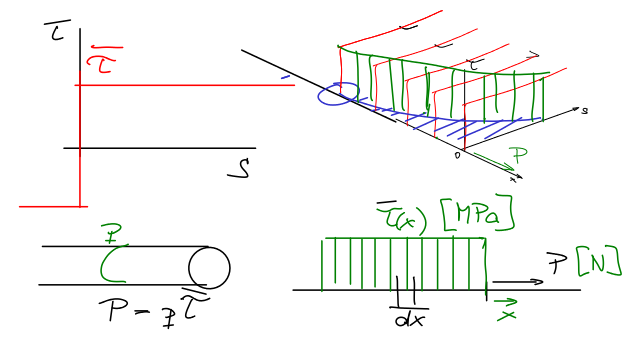
\includegraphics[width=0.7\textwidth]{drawings/constant_bond_boundary_conditions.png}
	\caption{Assumptions included in the pullout-model with constant bond stress}
	\label{FIGConstantBondAssumptions}
\end{figure}

\subsection{Constant shear bond to a rigid matrix}

\label{SEC:ConstantBondRigidMatrix}

\mnote{Just one unknown field $u_\mathrm{f}(x)$}
Regarding an infinitesimal element of an interface area within a composite cross section shown in Fig.~\ref{FIGConstantBondVariables} we can formulate the local equilibrium condition as
\begin{figure}[ht]
	\centering
  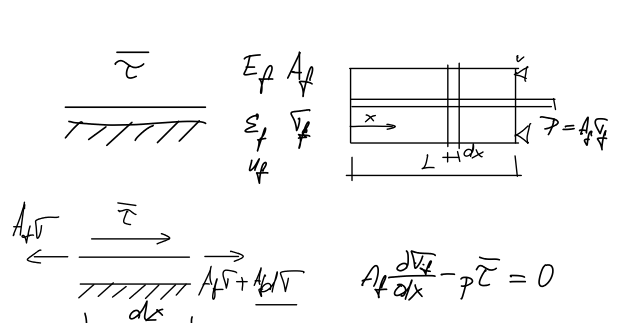
\includegraphics[width=0.7\textwidth]{drawings/constant_bond_variables.png}
	\caption{Variables and parameters describing the constant bond model}
	\label{FIGConstantBondVariables}
\end{figure}
\begin{equation} \label{eq:equilibrium}
A_\ifilam \; \sigma_{\ifilam,x} - p \bar{\tau} =0
\end{equation}
\mnote{Local equilibrium}
where 
$A_\ifilam$ is the area of the reinforcement, $\sigma_{\ifilam,x}$ the derivative of the fiber stress with respect to the the length coordinate $x$, $p$ is the perimeter, and $\bar{\tau}$ stands for the constant shear/frictional bond stress.
Integration of Eq.~(\ref{eq:equilibrium}) reveals that the stress $\sigma(x)$ is linear, i.e.
\begin{align}
\label{eq:stress_1}
\sigma_{\ifilam}(x) = \frac{p \bar{\tau}}{A_{\ifilam}} x + C
\end{align}
Assuming a linear elastic reinforcement behavior with the material stiffness $E_\ifilam$ 
at every point $x$ of the reinforcement
($\sigma_\ifilam = E_\ifilam \varepsilon_\ifilam$) we rewrite this condition 
for strain along the debonded zone as
\begin{align}
\label{eq:strain_1}
\varepsilon_{\ifilam}(x) &= \frac{1}{E_\ifilam} \sigma_{\ifilam}(x) = 
\frac{1}{E_\ifilam} \left( \frac{p \bar{\tau}}{A_{\ifilam}} x + C \right)
\end{align}
\mnote{Kinematics}
and then into the kinematic condition
\begin{align}
\label{eq:const_shear_displ}
u_{\ifilam} = \int \varepsilon_\ifilam(x) \, \mathrm{d}x = 
\frac{1}{E_\ifilam} \left( \frac{p \bar{\tau}}{2A_{\ifilam}} x^2 + Cx \right)  + D
=
\frac{1}{2}
\frac{p \bar{\tau}}{E_\ifilam A_{\ifilam}} x^2 + \frac{1}{E_\ifilam} C x + D
\end{align}
we obtain the quadratic function of the reinforcement displacement
with the two parameters $C,D$ to be determined using the boundary conditions.

\mnote{Resolve constants}
To determine the constant $C$ we recall that the force distribution  along the bar given as
\begin{equation} \label{eq:Force}
F_\ifilam(x)  = \sigma_\ifilam (x)  A_\ifilam =  p \bar{\tau} x + C A_\ifilam,
\end{equation}  
must be equal to the applied load $P$ at the pulled end ($x=0$), i.e.
\begin{equation} \label{eq:Force_1}
F(0) = \sigma_\ifilam (0)  A_\ifilam = P \qquad  \implies \qquad   C = P/A_\ifilam.
\end{equation}
\mnote{Global equilibrium}
By substituting  Eq.~(\ref{eq:Force_1}) into Eq.~(\ref{eq:const_shear_displ}) 
the displacement field of the reinforcement can be rewritten as
\begin{align} 
u_\ifilam(x) = 
\frac{1}{2}
\frac{p \bar{\tau}}{E_\ifilam A_{\ifilam}} x^2 - \frac{P}{E_\ifilam A_\ifilam} x + D.
\label{eq:displacement_3}
\end{align}
To factor out the parameter $D$ another condition is needed. This condition can be introduced
by realizing that in zones, where the reinforcement is still bonded to the matrix, there is no slip and, thus, 
the displacement in the reinforcement at point $a$ is zero.  
\mnote{Compatibility}
Knowing that the debonded zone starts from the loaded end and propagates
inwards through the bond layer, we can require
\begin{align} 
u_\ifilam(a) & = 0
  \qquad  \implies \qquad
D = - \frac{a}{2 A_\mathrm{f} E_\mathrm{f}} (2P + ap\tau)
\label{eq:displacement_4}
\end{align}
Still, the problem has one unknown variable, namely the debonded length $a$. To resolve it, we need another condition. Realizing that also the strain at $a$ must vanish we can substitute $a$ for $x$ in Eq.~(\ref{eq:strain_1}) and resolve for the state variable $a$ to get
\begin{align}
\varepsilon_\ifilam(a) = 0  \qquad  \implies \qquad  a = -\frac{P}{p \bar{\tau}}  \label{eq:strain_4}.
\end{align}
\mnote{State fields}
With all the variables at hand, the sought reinforcement displacement corresponding to the given boundary conditions has the form
\begin{equation} \label{eq:displacement_5}
u_\ifilam(x) = 
\frac{1}{2}
\frac{p \bar{\tau}}{E_\ifilam A_{\ifilam}} x^2 - \frac{P}{E_\ifilam A_\ifilam} x + 
\frac{1}{2 E_\ifilam A_\ifilam} \frac{P^2}{p \bar{\tau}}.
\end{equation} 
Particularly interesting is the  displacement at the loaded end $u(x=0)$
\begin{equation} \label{eq:displacement_6}
u_\ifilam(0)= w = \frac{1}{2} \frac{P^2}{p \bar{\tau} E_\ifilam A_\ifilam} .
\end{equation}
\mnote{Pullout curve}
By solving this equation for $P$ we finally obtain an explicit function describing the pull-out curve in the form
\begin{equation} \label{eq:pullout}
P(w)= \sqrt{2  p \bar{\tau} E_\ifilam A_\ifilam w }.
\end{equation}

\begin{bmcsex}{Pullout from rigid matrix}{e21_pullout_from_rigid_matrix}
\paragraph{Question:} Consider the pullout test depicted in Fig.~\ref{fig_pull-out_rilem}.
Evaluate the pullout curve assuming that there is deformation in concrete
and that the bond behavior corresponds to the purely frictional bond
derived previously. The boundary value problem idealizing such structural
behavior is depicted in Fig.~\ref{fig_pull-out_rigid_matrix}ab.

\paragraph{Solution:} 
A python script evaluating the problem using the derived model (\ref{eq:pullout}) 
has been prepared \href{http://localhost:8888/tree/Examples/2_1_pullout_from_rigid_matrix.ipynb}{here}
to perform calculations using the model. It can be readily used to test the model and evaluate the pullout curves and also the stress, strain and displacement fields.
Exemplified results are provided here for the values of parameters
\begin{align}
    E_\mathrm{f} = 1, \;\; 
    A_\mathrm{f} = 1, \;\;
    \bar{\tau} = 1, \;\;
    L_\mathrm{b} = 1
\end{align}
\paragraph{Results:} The top-left diagram shows the $P(w)$ curve, 
the top right diagram shows the slip along the 
bond length for several load levels, 
the bottom diagrams visualize 
the strain and stress along the bond length.
Since $E_\mathrm{f}A_\mathrm{f} = 1$, they are equal.\\
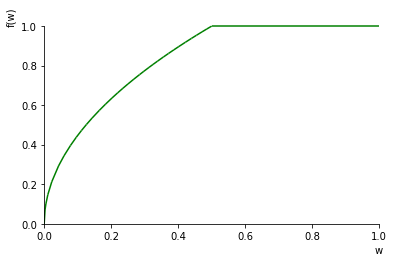
\includegraphics[clip,width=0.5\textwidth]
{bmcsex/ex21_pullout_from_rigid_matrix/ex21_pullout.png}
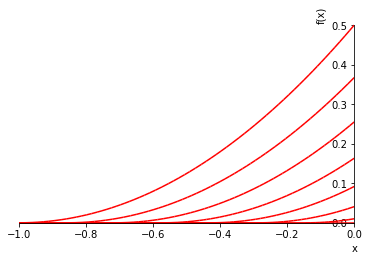
\includegraphics[clip,width=0.5\textwidth]
{bmcsex/ex21_pullout_from_rigid_matrix/ex21_slip_profile.png}
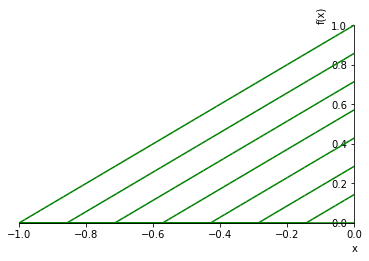
\includegraphics[clip,width=0.5\textwidth]
{bmcsex/ex21_pullout_from_rigid_matrix/ex21_strain_profile.png}
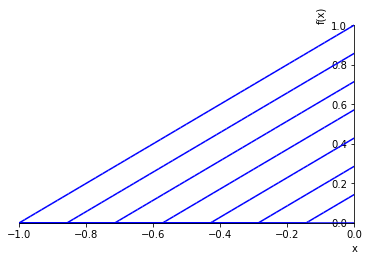
\includegraphics[clip,width=0.5\textwidth]
{bmcsex/ex21_pullout_from_rigid_matrix/ex21_stress_profile.png}

\paragraph{Task:} Change the material parameters given in the script to reproduce the test results of the RILEM pullout test presented in Fig.~\ref{fig_pull-out_rilem}. Is it possible to set up the model such that it can reproduce the results? 

\end{bmcsex}
\newpage
\begin{bmcsex}{Pullout from rigid matrix with extra bar length at the loaded end}{e22_pullout_from_rigid_matrix_extra_free_length}
\paragraph{Question:} The bar in test shown in Fig.~\ref{fig_pull-out_rilem}
does not start immediately at the beginning of the bonding zone. 
Extend the model by including the deformation of the bar along the free length 
such that it is possible to place the LVDT measuring 
the displacement on the steel bar at some distance from the bond zone.
In the evaluation use the parameters
\begin{align}
    E_\mathrm{f} = 1, \;\; 
    A_\mathrm{f} = 1, \;\;
    \bar{\tau} = 1, \;\;
    L_\mathrm{b} = 1, \;\;
    L_\mathrm{f} = 1
\end{align}

\paragraph{Solution:} 
The required extension of the analytical model requires another spring 
attached to the model previously derived and to impose a compatibility 
codition. The derivation has been done using 
the symbolic algebra package in the Python language.
The executable jupyter notebook can be downloaded  \href{https://moodle.rwth-aachen.de/pluginfile.php/261132/mod_folder/content/0/example_2.2_pullout_from_rigid_matrix_with_free_length.ipynb?forcedownload=1}{here}.

\paragraph{Results:} 
The diagrams demonstrate the difference with respect to Example~\ref{e21_pullout_from_rigid_matrix}
for $P(w)$ pullout curve, displacement, strain and stress fields along the bar.\\ 
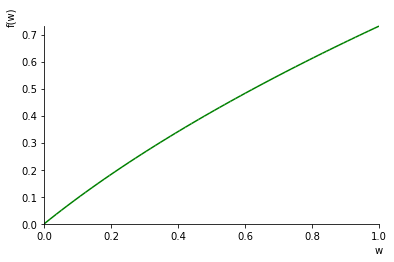
\includegraphics[clip,width=0.5\textwidth]
{bmcsex/ex22_Pullout_from_rigid_matrix_with_free_length/ex22_pullout.png}
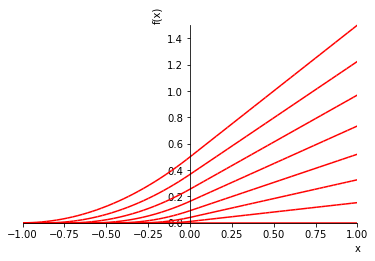
\includegraphics[clip,width=0.5\textwidth]
{bmcsex/ex22_Pullout_from_rigid_matrix_with_free_length/ex22_slip_profile.png}
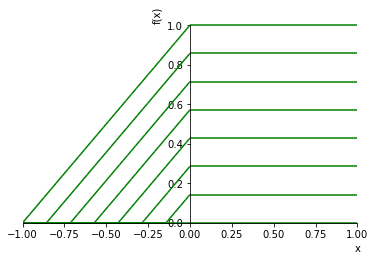
\includegraphics[,clip,width=0.5\textwidth]
{bmcsex/ex22_Pullout_from_rigid_matrix_with_free_length/ex22_strain_profile.png}
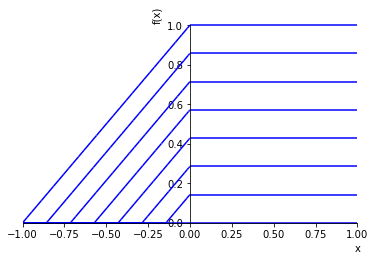
\includegraphics[clip,width=0.5\textwidth]
{bmcsex/ex22_Pullout_from_rigid_matrix_with_free_length/ex22_stress_profile.png}

\paragraph{Task:} Test the effect of the changing free bar length. How does the pullout curve $P(w)$ look like qualitatively if the free length of the bar gets very long? 

\paragraph{Task:} Name all possibilities how this pullout test can ultimately fail.

\end{bmcsex}

%\subfile{examples/e31_pullout_frictional/e31_pullout_frictional}

\subsection{Constant shear bond to elastic matrix}

\mnote{What if the matrix deforms as well?}

An extension of the previous model for elastic matrix can be done by refining the condition of compatibility.  
Let us exemplify this extension for two kinds of boundary conditions depicted in Fig.~\ref{fig_pull-out_em}.
\label{SEC:PullOutAnalyticalElasticMatrix}
Given the strain in the concrete matrix and in the fabric reinforcement, $\varepsilon_\mathrm{m}$ and $\varepsilon_\mathrm{f}$, respectively we can evaluate the relative slip at $x = 0 $ as
\begin{align}
    w = \int_{-a}^{0} \varepsilon_\mathrm{f} - \varepsilon_\mathrm{m} \, \mathrm{d}x.  
\end{align}

\begin{figure}[ht]
	\centering
  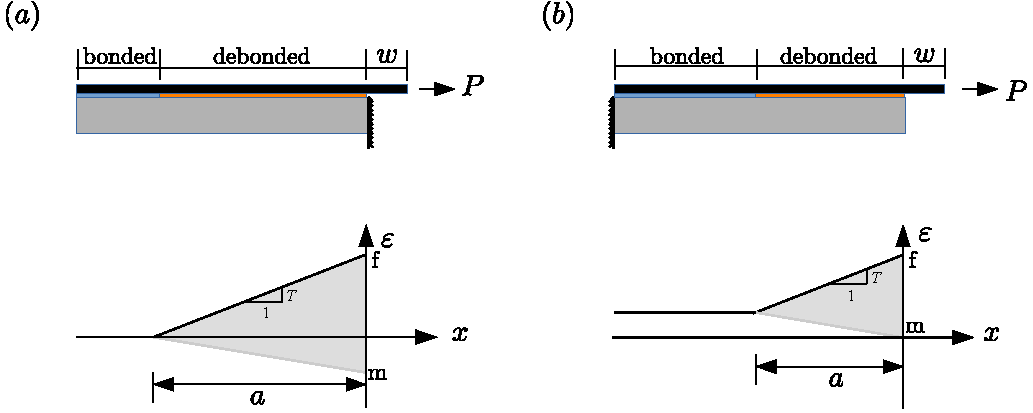
\includegraphics[width=0.9\textwidth]{fig/pull-out_em.pdf}
	\caption{Profile of strains in the pullout-model with constant bond stress; a) Matrix supported at loaded end, b) Matrix supported at unloaded end}
	\label{fig_pull-out_em}
\end{figure}

It is represented by the shaded area in Fig.~\ref{fig_pull-out_em}. In the simple case of constant bond, the area is of triangular shape so that the derivation can be simplified. In order to determine the area of the triangle, the following parameters are required: the strains $\varepsilon_\mathrm{f}(x=0)$ and $\varepsilon_\mathrm{m}(x=0)$, as well as the debonded length $a$. 

\subsubsection{Matrix supported at the loaded end (BC1)}
When the matrix is fixed at $x=0$ as shown in Fig.\ref{fig_pull-out_em}a,  the required parameters can be determined as
\begin{align}
   \varepsilon_\mathrm{f}(0) &= \frac{P}{E_\ifilam A_\ifilam},  \;\;
    \varepsilon_\mathrm{m}(0) = \frac{-P}{E_\mathrm{m} A_\mathrm{m}} \\
    T &= \frac{p\tau}{E_\ifilam A_\ifilam} \\
     a &= \frac{\varepsilon_\mathrm{f}(0)}{T} = \frac{P}{p\tau}.
\end{align}
Thus, the crack opening can be expressed as the area of the triangle
\begin{align}
   w &= \frac{1}{2}\left[\varepsilon_\mathrm{f}(0) - \varepsilon_\mathrm{m}(0)\right]a \nonumber \\
     &= \frac{1}{2}\frac{P^2}{p\tau} \left[\frac{1}{E_\ifilam A_\ifilam} + \frac{1}{E_\mathrm{m} A_\mathrm{m}}\right].
\end{align}
By solving this equation for $P$ we obtain the pullout curve in the form
\begin{align}
   P(w) = \sqrt{2wp\tau \frac{E_\mathrm{f}A_\mathrm{f}E_\mathrm{m}A_\mathrm{m}}{E_\mathrm{f}A_\mathrm{f}+E_\mathrm{m}A_\mathrm{m}}}.
\end{align}

\begin{bmcsex}{Pullout from elastic matrix clamped right}{e23_pullout_from_elastic_matrix_clamped_right}
Pullout from rigid matrix with extra bar length at the loaded 
The described procedure can be applied with further extensions considering different position of supports, inclusion of free-length of the reinforcement at the pulled-out end. The script containing this model is provided 
\href{https://moodle.rwth-aachen.de/pluginfile.php/261132/mod_folder/content/0/example_2.3_pull-out_from_elastic_matrix_supported_at_loaded_end.ipynb?forcedownload=1}{here}.

\paragraph{Task:} Use the model with the material parameters appropriate to carbon reinforcement and concrete with the stiffness $E_\mathrm{m} = 28$~GPa and find out for which ratio of cross-sectional areas $A_\mathrm{m}/A_\mathrm{m}$ 
does the pull-out curve change. 

\end{bmcsex}

\subsubsection{Matrix supported at unloaded end (BC2)}
For the case shown in Fig.\ref{fig_pull-out_em}b where the matrix is fixed at the left side, the values of $\varepsilon_\mathrm{f}(x=0)$ and $T$ remain the same, while
\begin{align}
   \varepsilon_\mathrm{m}(x=0) &= 0 \\
   \varepsilon_\mathrm{f}(x=-a) &= \frac{P}{E_\mathrm{f}(A_\mathrm{m}+A_\mathrm{f})},
\end{align}
and the debonded length
\begin{align}
      a &= \frac{\varepsilon_\mathrm{f}(x=0) - \varepsilon_\mathrm{f}(x=-a)}{T} \\
    &= \frac{P A_\mathrm{m}}{p\tau (A_\mathrm{f}+A_\mathrm{m})}.
\end{align}
Then the slip at $x=0$ can be written as 
\begin{align}
      w = \frac{1}{2}\frac{P^2A_\mathrm{m}}{p\tau E_\mathrm{f}A_\mathrm{f}(A_\mathrm{f}+A_\mathrm{m})}
\end{align}
and finally the pull-out response is given by
\begin{align}
      P(w) =  \sqrt{2wp\tau \frac{E_\mathrm{f}A_\mathrm{f}(A_\mathrm{f}+A_\mathrm{m})}{A_\mathrm{m}}}
\end{align}

\begin{bmcsex}{Pullout from elastic matrix clamped left}{e24_pullout_from_elastic_matrix_clamped_left}
Pullout from rigid matrix with extra bar length at the loaded 
The described procedure can be applied with further extensions considering different position of supports, inclusion of free-length of the reinforcement at the pulled-out end. The script containing this model is provided 
\href{https://moodle.rwth-aachen.de/pluginfile.php/261132/mod_folder/content/0/example_2.4_pull-out_from_elastic_matrix_supported_at_the_unloaded_end.ipynb?forcedownload=1}{here}.

\paragraph{Task:} Use the model with the material parameters appropriate to carbon reinforcement and concrete with the stiffness $E_\mathrm{f} = 28~GPa$ and find out for which ratio of cross-sectional areas $A_\mathrm{m}/A_\mathrm{m}$ 
does the pull-out curve change.
\paragraph{Task:} Answer the question: Assuming steel rebar, at which level of reinforcement ratio does the elasticity of matrix change the maximum pullout force by 10\% compared to the case of rigid matrix? 

\end{bmcsex}

\begin{bmcsex}{Pullout of a short fiber with decreasing bond length}{e25_pullout_of_short_fiber}
Pullout from rigid matrix with extra bar length at the loaded 
The described procedure can be applied with further extensions considering different position of supports, inclusion of free-length of the reinforcement at the pulled-out end. The script containing this model is provided 
\href{http://localhost:8888/tree/Examples/2_5_Pullout_from_rigid_matrix_with_a_fiber_of_finite_length.ipynb}{here}.

\paragraph{Task:} Use the model with the material parameters appropriate to carbon reinforcement and concrete with the stiffness $E_\mathrm{f} = 28~GPa$ and find out for which ratio of cross-sectional areas $A_\mathrm{m}/A_\mathrm{m}$ 
does the pull-out curve change.
\paragraph{Task:} Answer the question: Assuming steel rebar, at which level of reinforcement ratio does the elasticity of matrix change the maximum pullout force by 10\% compared to the case of rigid matrix? 

\end{bmcsex}

\subsection{Piecewise linear bond-slip law}

Besides the case of the frictional model, analytical solution can be derived also for linear-elastic bond as presented in \cite{one}
\stext{Can I correct the citation number? one?}
\begin{align}
    \label{eq:linear_bond_analytical}
    P(u_{\ifilam,0}) = 
    \frac{k \tanh(\alpha L)}
    {\alpha}u_{\ifilam,0}, \;\; \mathrm{with}\;
    \alpha = \sqrt{ pk
    \left(
    \frac{1}{E_\ifilam A_\ifilam}
    +
    \frac{1}{E_\imatrix A_\imatrix}
    \right)}
\end{align}

This solution can describe the initial stages up to the onset of debonding.
Notice that the relation the function $P(w)$ is linear.
This solution can be generalized for piecewise linear bond-slip law as exemplified in \cite{yuan_full-range_2004}. Then a solution of the pullout problem with 
non-linear bond-slip law can obtained by putting together the analytical solutions 
along every segment. However, a more general and efficient solution can be obtained
within the framework of the standard non-linear finite element solver. In the following 
chapter such a solver will be presented including the executable code to solve examples. 

\section{Conclusions and remarks}
This class of pull-out models is particularly useful as a basic component of models studying statistical 
aspects of scatter in heterogeneous materials in the vicinity of crack bridges.

\end{document}